%--------- Modify the following three lines for every homework
\def\yourid{yourid}
\def\collabs{list your collaborators}
\def\sources{list your sources}

% --- Do not modify the lines in this section-------------------------------------------------
\def\duedate{December 5, 2023 at 11:59 PM}
\def\pnumber{5}
\newcommand{\soln}{\medskip\noindent\textbf{Solution:}\vspace*{1ex}}

\documentclass[10pt]{article}
\usepackage{dsa2}

\usepackage{pbox}
\usepackage{tikz}
\usetikzlibrary{arrows}

\begin{document}
\thispagestyle{empty}
\handout


%--- Beginning of the problems.  Students should look for the TODO comment after each problem
%--- and add their answers there.

%===============================================================================================


\begin{problem} Max Flow \end{problem}

\noindent Given the following Flow Network $G$ and Residual Graph $G'$:

\vskip 2em
\begin{center}
\resizebox{.45\textwidth}{!}{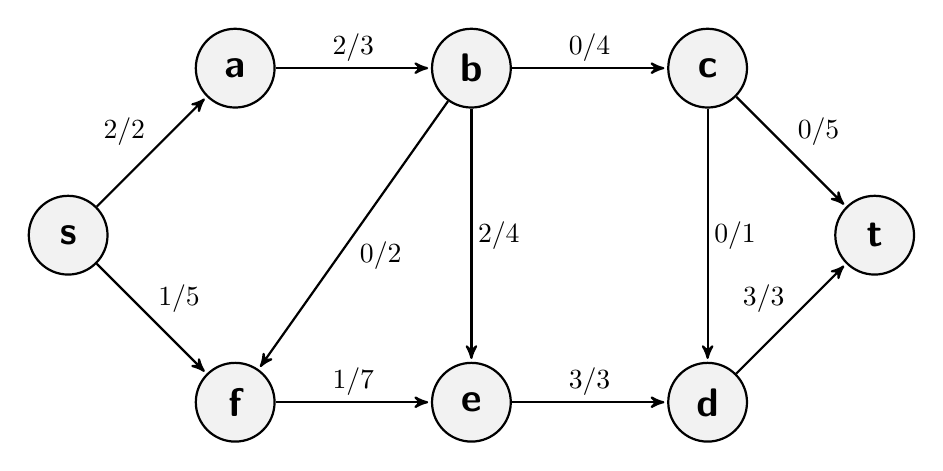
\begin{tikzpicture}[->,>=stealth',shorten >=1pt,auto,node distance=3cm,
  thick,main node/.style={circle,fill=gray!10,draw,
  font=\sffamily\Large\bfseries,minimum size=10mm}]

  \node[main node] (s) {s};
  \node[main node] (a) [above right of=s] {a};
  \node[main node] (b) [right of=a] {b};
  \node[main node] (c) [right of=b] {c};
  \node[main node] (t) [below right of=c] {t};
  \node[main node] (f) [below right of=s] {f};
  \node[main node] (e) [right of=f] {e};
  \node[main node] (d) [right of=e] {d};

  \path[every node/.style={
        fill=white,inner sep=2pt}]
    % Right-hand-side arrows rendered from top to bottom to
    % achieve proper rendering of labels over arrows.
    (s) edge [] node[] {2/2} (a)
        edge [] node[] {1/5} (f)
    (a) edge [] node[] {2/3} (b)
    (b) edge [] node[] {0/4} (c)
        edge [] node[] {0/2} (f)
        edge [] node[] {2/4} (e)
    (c) edge [] node[] {0/5} (t)
        edge [] node[] {0/1} (d)
    (f) edge [] node[] {1/7} (e)
    (e) edge [] node[] {3/3} (d)
    (d) edge [] node[] {3/3} (t);
\end{tikzpicture}}\hfill
\resizebox{.45\textwidth}{!}{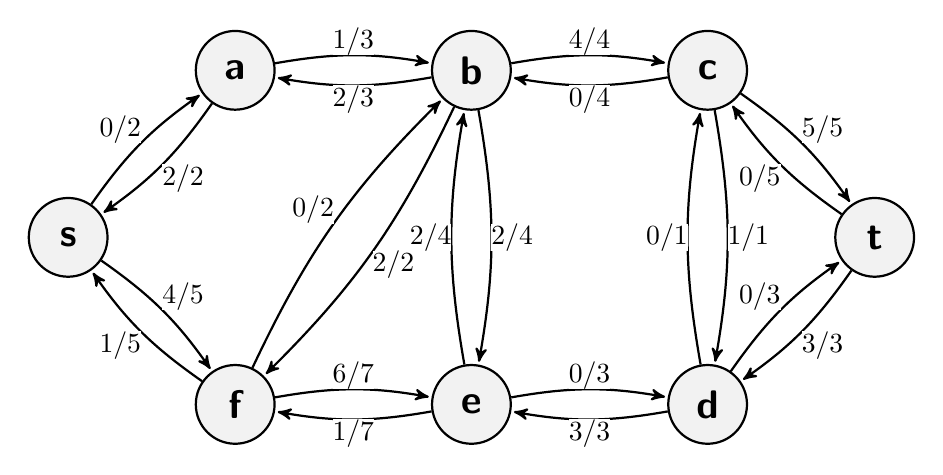
\begin{tikzpicture}[->,>=stealth',shorten >=1pt,auto,node distance=3cm,
  thick,main node/.style={circle,fill=gray!10,draw,
  font=\sffamily\Large\bfseries,minimum size=10mm}]

  \node[main node] (s) {s};
  \node[main node] (a) [above right of=s] {a};
  \node[main node] (b) [right of=a] {b};
  \node[main node] (c) [right of=b] {c};
  \node[main node] (t) [below right of=c] {t};
  \node[main node] (f) [below right of=s] {f};
  \node[main node] (e) [right of=f] {e};
  \node[main node] (d) [right of=e] {d};

  \path[every node/.style={
        fill=white,inner sep=0pt,outer sep=0pt}]
    % Right-hand-side arrows rendered from top to bottom to
    % achieve proper rendering of labels over arrows.
    (s) edge [bend left=10] node[] {0/2} (a)
        edge [bend left=10] node[] {4/5} (f)
    (a) edge [bend left=10] node[] {2/2} (s)
        edge [bend left=10] node[] {1/3} (b)
    (b) edge [bend left=10] node[] {2/3} (a)
        edge [bend left=10] node[] {4/4} (c)
        edge [bend left=10] node[] {2/2} (f)
        edge [bend left=10] node[] {2/4} (e)
    (c) edge [bend left=10] node[] {5/5} (t)
        edge [bend left=10] node[] {0/4} (b)
        edge [bend left=10] node[] {1/1} (d)
    (f) edge [bend left=10] node[] {6/7} (e)
        edge [bend left=10] node[] {1/5} (s)
        edge [bend left=10] node[] {0/2} (b)
    (e) edge [bend left=10] node[] {0/3} (d)
        edge [bend left=10] node[] {2/4} (b)
        edge [bend left=10] node[] {1/7} (f)
    (d) edge [bend left=10] node[] {0/3} (t)
        edge [bend left=10] node[] {0/1} (c)
        edge [bend left=10] node[] {3/3} (e)
    (t) edge [bend left=10] node[] {0/5} (c)
        edge [bend left=10] node[] {3/3} (d)
    ;
\end{tikzpicture}}
\end{center}
\hspace{0.85in} Flow Network $G$ \hspace{2in} Residual Graph $G'$


\begin{enumerate}
    \item Find an augmenting path in the graph $G'$.  List the nodes in the path you found in order (e.g., $s\rightarrow a \rightarrow b \rightarrow c \rightarrow d \rightarrow t$).

    \soln
    
    \item Update the Flow Network $G$ above.  You \textbf{must} edit the graph below (do not upload a picture).
    
    \soln
    \begin{center}
    \resizebox{.45\textwidth}{!}{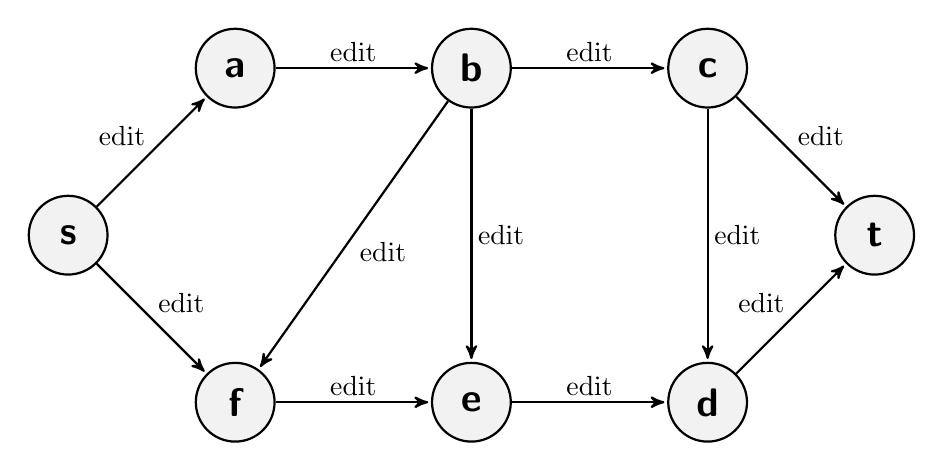
\begin{tikzpicture}[->,>=stealth',shorten >=1pt,auto,node distance=3cm,
      thick,main node/.style={circle,fill=gray!10,draw,
      font=\sffamily\Large\bfseries,minimum size=10mm}]

      %% THESE ARE THE NODES.  NOTE THAT THEY ARE LABELED IN LATEX
      \node[main node] (s) {s};
      \node[main node] (a) [above right of=s] {a};
      \node[main node] (b) [right of=a] {b};
      \node[main node] (c) [right of=b] {c};
      \node[main node] (t) [below right of=c] {t};
      \node[main node] (f) [below right of=s] {f};
      \node[main node] (e) [right of=f] {e};
      \node[main node] (d) [right of=e] {d};

      %% THESE ARE THE EDGES. UPDATE THE WEIGHTS BELOW.
      \path[every node/.style={
            fill=white,inner sep=2pt}]
            (s) edge [] node[] {edit} (a)
            edge [] node[] {edit} (f)
        (a) edge [] node[] {edit} (b)
        (b) edge [] node[] {edit} (c)
            edge [] node[] {edit} (f)
            edge [] node[] {edit} (e)
        (c) edge [] node[] {edit} (t)
            edge [] node[] {edit} (d)
        (f) edge [] node[] {edit} (e)
        (e) edge [] node[] {edit} (d)
        (d) edge [] node[] {edit} (t);
    \end{tikzpicture}}
    \end{center}
    
    \item Find the min cut of the graph.  List the nodes on each side of the cut.
    
    \soln
    
\end{enumerate}


\newpage

\begin{problem} Element Uniqueness Reduction \end{problem}

Reduce Element Uniqueness to Mode in $O(n)$ time.  Element Uniqueness is defined as: given a list of numbers, return true if no number appears more than once (i.e., every number is distinct).  Mode is defined as: given a list of numbers, return one of the numbers which appears most frequently in the list; i.e. if everything was unique it will return an arbitrary element.

\soln

\newpage

\begin{problem} Reading and Evaluating Proofs \end{problem}

Generative AI systems are exciting -- \textit{and scary}. They can answer many questions, but how much can we trust the results?

For this problem you will choose an generative AI system (e.g., ChatGPT, Bing (inside of Edge)) and ask it to do a proof for an algorithm we've studied in this unit---specifically, the proof that the reduction of Bi-Partite Matching to Max-Flow is correct. You'll then carefully read the proof it gives you and compare it to the version of that proof in our textbook, noting any issues or significant differences. 

Here's a suggested prompt to give the system. You may use this unchanged, or alter it to try to get a better result.
\\
\textit{Answer this question as if you were a computer scientist. Formally prove that the Bi-Partite Matching algorithm using a max-flow algorithm is correct (i.e, it always find the optimal matching between nodes in the bi-partite graph).}



In your solution, provide the following;
\begin{enumerate}
\item Give the name and version number of the generative AI system you've used.

\soln

\item In a sentence, describe the proof strategy used by the AI.

\soln

\item Study the textbook's proof of this algorithm, Lemma 24.9 in Section 24.3 of the 4th edition of the textbook. In no more than 5 or 6 sentences, describe any issues or problems you see in the AI's result or how it differs from the textbook's proof.  \textit{Your answer might address the following questions: Do you think it successfully proves correctness?  Are there gaps or odd logical jumps in the proof it provides?  How different is it from the proof in the textbook?  (If there are no issues to report, just say that.)}

\soln

\item Copy the prompt you gave the AI below.

\soln

\item Copy the AI's response (the proof) below.

\soln

\end{enumerate}
    


\newpage

\begin{problem} Algorithms and Society: Ethical and Social Issues \end{problem}

In society the term \textit{algorithms} is frequently used for what some call \textit{algorithmic decision systems}.  These are systems that rely on large amounts of data and algorithms that use AI or machine learning to make decisions in a wide range of important issues in society.

\begin{center}
    \url{https://en.wikipedia.org/wiki/Automated_decision-making}
\end{center}

While these systems are different in nature that almost all the algorithms topics we've studied in this course, some kind of algorithmic process is at the heart of such systems. It is appropriate for a computing student studying algorithms to be aware of this use of the term and to understand examples of such systems and the social and ethical challenges they pose.

Below is a list of articles, etc., that touch on algorithm-based systems and social or ethical issues in society. 
Choose one article that interests you, and answer the following questions.
\begin{enumerate}
\item List the title of the of the reading that you chose.

\soln

\item In no more than five or six sentences, summarize how one algorithmic decision system discussed in the reading may lead to negative or undesirable consequences for individuals or societies. (The reading may discuss more than one, but you only need to write about one.)

\soln

\item In a few sentences, what actions do you think the computing personnel or organizations that create such systems could do to reduce possible negative or undesirable consequences?  (Keep your answers brief!)

\soln

\end{enumerate}

\vspace*{.35in}
\textbf{Readings (choose one):}
\begin{enumerate}

\item \textit{Bias in AI-based models for medical applications: challenges and mitigation strategies}
\\ \url{https://www.nature.com/articles/s41746-023-00858-z}

\item \textit{Machine Bias} (This is a longer article on risk assessments in criminal sentencing that got a lot of national attention.)
\\ \small{\url{https://www.propublica.org/article/machine-bias-risk-assessments-in-criminal-sentencing}}

\item \textit{Why colleges are using algorithms to determine financial aid levels}
\\ \small{\url{https://www.highereddive.com/news/colleges-enrollment-algorithms-aid-students/692601}}

\item \textit{Designing Ethical Self-Driving Cars}
\\ \url{https://hai.stanford.edu/news/designing-ethical-self-driving-cars}

\item \textit{Algorithms that Run the World, an interview with Cathy O’Neil} (author of the book "Weapons of Math Destruction")
\\ \small{\url{https://thedecisionlab.com/podcasts/algorithms-that-run-the-world-with-cathy-oneil}}

\end{enumerate}

\end{document}

